%----------------------------------------------------------------------------------------
%	PACKAGES AND OTHER DOCUMENT CONFIGURATIONS
%----------------------------------------------------------------------------------------

\documentclass[twoside]{article}

\usepackage{lipsum} % Package to generate dummy text throughout this template

\usepackage[sc]{mathpazo} % Use the Palatino font
\usepackage[T1]{fontenc} % Use 8-bit encoding that has 256 glyphs
\usepackage[utf8]{inputenc}
\linespread{1.05} % Line spacing - Palatino needs more space between lines
\usepackage{microtype} % Slightly tweak font spacing for aesthetics
\usepackage{graphicx}

\usepackage[hmarginratio=1:1,top=32mm,columnsep=20pt]{geometry} % Document margins
\usepackage{multicol} % Used for the two-column layout of the document
\usepackage[hang, small,labelfont=bf,up,textfont=it,up]{caption} % Custom captions under/above floats in tables or figures
\usepackage{booktabs} % Horizontal rules in tables
\usepackage{float} % Required for tables and figures in the multi-column environment - they need to be placed in specific locations with the [H] (e.g. \begin{table}[H])
\usepackage{hyperref} % For hyperlinks in the PDF

\usepackage{lettrine} % The lettrine is the first enlarged letter at the beginning of the text
\usepackage{paralist} % Used for the compactitem environment which makes bullet points with less space between them

\usepackage{abstract} % Allows abstract customization
\renewcommand{\abstractnamefont}{\normalfont\bfseries} % Set the "Abstract" text to bold
\renewcommand{\abstracttextfont}{\normalfont\small\itshape} % Set the abstract itself to small italic text

\usepackage{titlesec} % Allows customization of titles
\renewcommand\thesection{\Roman{section}} % Roman numerals for the sections
\renewcommand\thesubsection{\Roman{subsection}} % Roman numerals for subsections
\titleformat{\section}[block]{\large\scshape\centering}{\thesection.}{1em}{} % Change the look of the section titles
\titleformat{\subsection}[block]{\large}{\thesubsection.}{1em}{} % Change the look of the section titles

\usepackage{amsmath}
\usepackage{algpseudocode}
\usepackage{algorithm}


%----------------------------------------------------------------------------------------
%	TITLE SECTION
%----------------------------------------------------------------------------------------

\title{\vspace{-15mm}\fontsize{24pt}{10pt}\selectfont\textbf{Comparing k-NN and Logistic Regression algorithms for wine classification}}

\author{
\large
\textsc{Algorithms for classification of wine types and quality}\\[2mm]
\textsc{F\'{a}bio Pinheiro  \& Jo\~{a}o Duro}\\[2mm]
\vspace{-5mm}
}
\date{}

%----------------------------------------------------------------------------------------

\begin{document}

\maketitle % Insert title

%----------------------------------------------------------------------------------------
%	ABSTRACT
%----------------------------------------------------------------------------------------

\begin{abstract}

%\noindent \lipsum[1]

\end{abstract}
Com o almento do power computational começa a fazer sentido usar algoritons mais complaxesos para obetremos melhores resultados.

%----------------------------------------------------------------------------------------
%	ARTICLE CONTENTS
%----------------------------------------------------------------------------------------

\begin{multicols}{2} % Two-column layout throughout the main article text

\section{Introduction}
\indent \par
TODO
Something in this document. This paragraph contains no information 
and its purposes is to provide an example on how to insert white 
spaces and lines breaks.\\
Something in this document. This paragraph contains no information 
and its purposes is to provide an example on how to insert white 
spaces and lines breaks.\par
When a line break is inserted, the text is not indented, there 
are a couple of extra commands do line breaks. \newline
This paragraph provides no information whatsoever. We are exploring 
line breaks. \hfill \break
And combining two commands
%\lipsum[2-4]


%------------------------------------------------

\section{Methods}
\subsection*{Normalize data}

\subsection*{k-nearest neighbors algorithm (k-NN)}
\indent \par
k-nearest neighbors algorithm also known as k-NN is a non-parametric method used for classification and regression. In both cases the k-NN algorithm starts from the principle that similar data are
closed one to another. \par
The algorithm is just given a point '$Y$' to find the k points from training data where distance where is smaller that all the anthers. Then choose the class more frequent, in case of a tie, pick a random one random among the most frequented.

\subsubsection*{Euclidean Distance}
For n dimensions Euclidean Distance is give by following formula:
\[ d(p,q)= \sqrt{(p_1 - q_1)^2 + (p_2 - q_2)^2 + ... + (p_n - q_n)^2} \]
(Dimensions in here is the number of feature/parameters of the data)
\subsubsection*{???????? Distance}
TODO 
\subsection*{Logistic Regression}
\indent \par
"It is assumed that we have a series of N observed data points. Each data point i consists of a set of m explanatory variables $x_{1,i} x_{2,i} $ ... $x_{m,i}$ (also called independent variables, predictor variables, input variables, features, or attributes), and an associated binary-valued outcome variable $Y_i$ (also known as a dependent variable, response variable, output variable, outcome variable or class variable), i.e. it can assume only the two possible values "failure" or 1 "success". The goal of logistic regression is to explain the relationship between the explanatory variables and the outcome, so that an outcome can be predicted for a new set of explanatory variables."
%\lipsum[5-9]

%\begin{figure}[H]
%\centering
%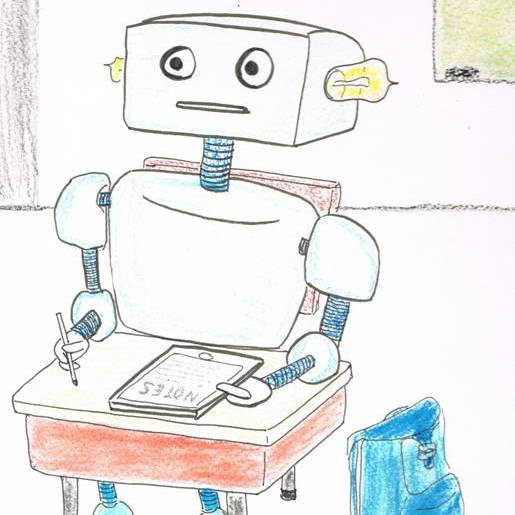
\includegraphics[width=0.5\textwidth]{learning}
%\caption{Learning is important but big processors are importanter. \cite{alpaydin2004introduction}}
%\label{fig:learning}
%\end{figure}

%------------------------------------------------

\section{Experiments}
\subsection*{Wine type:}
\indent \par
To classify the type of wine first we used the k-nearest neighbors algorithm.
To choose the K we separate the training dataset in two set (3750 points for training and points 1250 points for validation). \par
After to improve the results we try to use the some method but with the data normalize. 

\subsection*{Wine quality}
F



%------------------------------------------------

\section{Results}

\begin{itemize}
  \item Number of parameters: 11
  \item Number of samples in training set: $5000$?
  \item Number of samples in test set: $1000$
  \item \#Red: $906$
  \item \#White: $4094$
  \item \#Q1: $5$
  \item \#Q2: $161$
  \item \#Q3: $854$
  \item \#Q4: $2197$
  \item \#Q5: $1604$
  \item \#Q6: $159$
  \item \#Q7: $20$
\end{itemize}



\begin{table}[H]
\caption{My current knowledge of tables}
\centering
\begin{tabular}{cc}
\textbf{Table type} & \textbf{Likely location}\\
\midrule
Coffee table & Living room\\
Dining table & Dining room\\
Bedside table & Bedroom
\end{tabular}
\end{table}

\subsection{Confusion matrix for the wine quality}

\begin{table}[H]
\caption{Using k-NN with k=1}
\centering
\begin{tabular}{r||c|c|c|c|c|c|c}
\textbf{Quality} & \textbf{1} & \textbf{2} & \textbf{3} & \textbf{4} & \textbf{5} & \textbf{6} & \textbf{7}\\
\hline \hline
\textbf{1} & 0 & 0 & 0 & 0 & 0 & 0 & 0	\\
\hline
\textbf{2} & 0 & 13 & 7 & 5 & 1 & 0 & 0\\
\hline
\textbf{3} & 0 & 9 & 114 & 49 & 9 & 0 & 0\\
\hline
\textbf{4} & 0 & 6 & 44 & 272 & 78 & 8 & 0\\
\hline
\textbf{5} & 0 & 0 & 11 & 99 & 225 & 9 & 0\\
\hline
\textbf{6} & 0 & 0 & 3 & 11 & 12 & 10 & 0\\
\hline
\textbf{7} & 0 & 0 & 0 & 1 & 3 & 1 & 0\\
\end{tabular}
\end{table}




\begin{table}[H]
\caption{Using logistic regression}
\centering
\begin{tabular}{r||c|c|c|c|c|c|c}
\textbf{Quality} & \textbf{1} & \textbf{2} & \textbf{3} & \textbf{4} & \textbf{5} & \textbf{6} & \textbf{7}\\
\hline \hline
\textbf{1} & a & b & c & d & f & g & i\\
\hline
\textbf{2} & a & b & c & d & f & g & i\\
\hline
\textbf{3} & a & b & c & d & f & g & i\\
\hline
\textbf{4} & a & b & c & d & f & g & i\\
\hline
\textbf{5} & a & b & c & d & f & g & i\\
\hline
\textbf{6} & a & b & c & d & f & g & i\\
\hline
\textbf{7} & a & b & c & d & f & g & i\\
\end{tabular}
\end{table}
%\lipsum[12-14]


%------------------------------------------------

\section{Discussion}

space and computers power
espaço ocupado pelo knn e pelo logistic regresion

The values of quality are not independent with this a mean if a wine and classify was quality '$x$' with is not the correct one, but is much more probably that the right quality is $x-1$ or $x+1$ than be $x-2$, $x+2$, $x-3$, $x+3$ ... \\
We could have used this to classify the quality of wine.


One of the motives for the result be soo low for the quality of one wine is a subjective thing, two wine enthusiasts do not necessary give the same qualification for the same wine. This way it would be interesting to compare the result our classifier with two independent groups of human wine enthusiasts for each wine. Since the quality is a subjective we would expect the error between our result and the human result should be close to the error between the two independent groups of humans.





k par and k odd 
%\lipsum[15-16]


%----------------------------------------------------------------------------------------
%	REFERENCE LIST
%----------------------------------------------------------------------------------------

\bibliographystyle{plain}
\bibliography{final_report}{}
%------------------------------------------------

\section*{Appendix A}

%\lipsum[17]

%----------------------------------------------------------------------------------------

\end{multicols}

\end{document}
